\chapter{Determinants}\label{elementarydeterminants}
\chaptermark{Determinants}

Given a square matrix, is there an easy way to know when it is invertible?  Answering this fundamental question is 
the goal of this chapter.

\section{The Determinant Formula}

The determinant boils down a square matrix to a a single number. That number determines whether the square matrix is invertible or not.  
Lets see how this works for small matrices first.

\subsection{Simple Examples}

For small cases, we already know when a matrix is invertible.  If $M$ is a $1\times 1$ matrix, then $M=(m) \Rightarrow M^{-1}=(1/m)$.  Then $M$ is invertible if and only if $m\neq 0$.

\vspace{.3cm}

For $M$ a $2\times 2$ matrix, chapter~\ref{Matrices} section~\ref{inverse_matrix} shows that if \[M=\begin{pmatrix}
m^1_1 & m^1_2 \\[1mm]
m^2_1 & m^2_2 \\
\end{pmatrix}\, ,\] then \[M^{-1}=\frac{1}{m^1_1m^2_2-m^1_2m^2_1}\begin{pmatrix}
m^2_2 & -m^1_2 \\[1mm]
-m^2_1 & m^1_1 \\
\end{pmatrix}\, .\] Thus $M$ is invertible if and only if 
\vspace{.3cm}

\[m^1_1m^2_2-m^1_2m^2_1\neq 0\, .\]  For $2\times 2$ matrices, this quantity is called the \emph{determinant of $M$}\index{Determinant!$2\times 2$ matrix}.
\[
\det M = \det \begin{pmatrix}
m^1_1 & m^1_2 \\[1mm]
m^2_1 & m^2_2 \\
\end{pmatrix} = m^1_1m^2_2-m^1_2m^2_1\, .
\]

\begin{figure}
\begin{center}
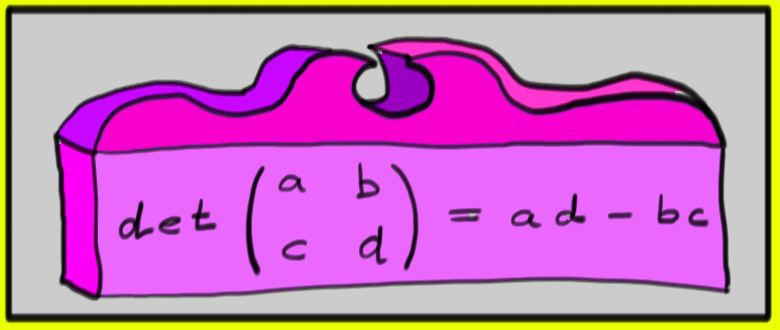
\includegraphics[scale=.35]{\elemMatDetPath/det2x2.jpg}
\end{center}
\caption{Memorize the determinant formula for a 2$\times$2 matrix!}
\end{figure}


\begin{example}
For a $3\times 3$ matrix, \[M=\begin{pmatrix}
m^1_1 & m^1_2 & m^1_3\\[1mm]
m^2_1 & m^2_2 & m^2_3\\[1mm]
m^3_1 & m^3_2 & m^3_3\\
\end{pmatrix}\, ,\] then---see \hyperref[det33]{review question}~\ref{det33}---$M$ is non-singular if and only if\index{Determinant!$3\times 3$ matrix}:
\vspace{.1cm}
\[
\det M= 
m^1_1m^2_2m^3_3 
- m^1_1m^2_3m^3_2 
+ m^1_2m^2_3m^3_1
- m^1_2m^2_1m^3_3  
+ m^1_3m^2_1m^3_2
- m^1_3m^2_2m^3_1
\neq 0.
\]

\noindent
Notice that in the subscripts, each ordering of the numbers $1$, $2$, and $3$ occurs exactly once.  Each of these is a \emph{permutation} of the set $\{1,2,3\}$.
\end{example}



\subsection{Permutations}
Consider $n$ objects labeled $1$ through $n$ and shuffle them.  Each possible shuffle is called a \emph{permutation}\index{Permutation}.  
For example, here is an example of a permutation of $1$--$5$:
\[
\sigma = \begin{bmatrix}
1 & 2 & 3 & 4 & 5 \\
4 & 2 & 5 & 1 & 3 
\end{bmatrix}
\]
We can consider a permutation $\sigma$ as an invertible function from the set of numbers $[n] := \{1, 2, \dotsc, n\}$ to $[n]$, so can  write $\sigma(3) = 5$ in the above example. In general we can write
\[\left[\!
\begin{array}{ccccc}
1 & 2 & 3 & 4 & 5 \\[1mm]
\sigma(1) & \sigma(2) & \sigma(3) & \sigma(4) & \sigma(5)
\end{array}\!\right]\, ,
\]
but since the top line of any permutation is always the same, we can omit it and just write:
\[
\sigma = \begin{bmatrix}
\sigma(1) & \sigma(2) & \sigma(3) & \sigma(4) & \sigma(5)
\end{bmatrix}
\]
and so our example becomes simply  $\sigma = [4\, 2\, 5\, 1\, 3]$. 
%There is also one more notation called cycle notation, but we do not discuss it here.

The mathematics of permutations is extensive; there are a few key properties of permutations that we'll need:

\begin{itemize}
\item There are $n!$ permutations of $n$ distinct objects, since there are $n$ choices for the first object, $n-1$ choices for the second once the first has been chosen, and so on.

\item Every permutation can be built up by successively swapping pairs of objects.  For example, to build up the permutation $\begin{bmatrix} 3 & 1 & 2 \end{bmatrix}$ from the trivial permutation $\begin{bmatrix} 1 & 2 & 3 \end{bmatrix}$, you can first swap $2$ and $3$, and then swap $1$ and $3$.

\item \hypertarget{permutation_parity}{For any given} permutation $\sigma$, there is some number of swaps it takes to build up the permutation.  (It's simplest to use the minimum number of swaps, but you don't have to: it turns out that \emph{any} way of building up the permutation from swaps will have have the same parity of swaps, either even or odd.) 
If this number happens to be even, then $\sigma$ is called an \emph{even permutation};\index{Even permutation} if this number is odd, then $\sigma$ is an \emph{odd permutation}\index{Odd permutation}.  In fact, $n!$ is even for all $n\geq 2$, and exactly half of the permutations are even and the other half are odd.  It's worth noting that the trivial permutation (which sends $i\rightarrow i$ for every $i$) is an even permutation, since it uses zero swaps.
\end{itemize}

\begin{definition}
The {\bfseries sign function}\index{Sign function} is a function $\text{sgn}$ that sends permutations to the set $\{-1,1\}$ with rule of correspondence defined by
\[ \text{sgn}(\sigma) = 
\left\{ \begin{array}{rl}
1 & \mbox{if $\sigma$ is even}\\
-1 & \mbox{if $\sigma$ is odd}.\end{array} \right.
\]
\end{definition}

%For more on the swaps (also known as inversions) and the sign function, see \hyperref[prob_inversion_number]{Problem~\ref*{prob_inversion_number}}.

\Videoscriptlink{elementary_matrices_permutations.mp4}{Permutation Example}{scripts_elementary_matrices_permutations}

%\begin{center}\href{\webworkurl ReadingHomework12/1/}{Reading homework: problem 12.1}\end{center}
\Reading{Determinants}{1}

We can use permutations to give a definition of the determinant.

\begin{definition}  The {\bfseries determinant}\index{Determinant} of $n \times n$ matrix $M$ is 
\begin{center}
\scalebox{1.2}{
\shabox{
$
\det M = {\textstyle \sum\limits_{\sigma}}\  \text{sgn}(\sigma)\,  m^1_{\sigma(1)}m^2_{\sigma(2)}\cdots m^n_{\sigma(n)}.
$
}}\end{center}
\end{definition}
The sum is over all permutations of $n$ objects; a sum over the all elements of $\{ \sigma: \{1,\dots,n\}\to  \{1,\dots,n\}\}$.  Each summand is a product of n entries from the matrix  with each factor from a different row. 
In different terms of the sum the column numbers are shuffled by different permutations~$\sigma$.

The last statement about the summands yields a nice property of the determinant:
\begin{theorem}
If $M=(m^i_j)$ has a row consisting entirely of zeros, then $m^i_{\sigma(i)}=0$ for every $\sigma$ and some $i$.  Moreover
$\det M=0$.
\end{theorem}


\begin{example}
Because there are many permutations of $n$, writing the determinant this way for a general matrix gives a very long sum.  For $n=4$, there are $24=4!$ permutations, and for $n=5$, there are already $120=5!$ permutations.\\

\noindent
For a $4\times 4$ matrix, $M=\begin{pmatrix}
m^1_1 & m^1_2 & m^1_3 & m^1_4\\[1mm]
m^2_1 & m^2_2 & m^2_3 & m^2_4\\[1mm]
m^3_1 & m^3_2 & m^3_3 & m^3_4\\[1mm]
m^4_1 & m^4_2 & m^4_3 & m^4_4\\
\end{pmatrix}$, then $\det M$ is:
\begin{eqnarray*}
\det M &=& 
 m^1_1m^2_2m^3_3m^4_4
-m^1_1m^2_3m^3_2m^4_4
-m^1_1m^2_2m^3_4m^4_3 \\[1mm]
& -&m^1_2m^2_1m^3_3m^4_4
+m^1_1m^2_3m^3_4m^4_2
+m^1_1m^2_4m^3_2m^4_3 \\[1mm]
&+ & m^1_2m^2_3m^3_1m^4_4
+m^1_2m^2_1m^3_4m^4_3
\pm \text{16 more terms}.
\end{eqnarray*}
\end{example}
This is very cumbersome.

Luckily, it is very easy to compute the determinants of certain matrices.  For example, if $M$ is diagonal, meaning that $M^i_j=0$ whenever $i\neq j$,  then all summands of the determinant involving off-diagonal entries vanish and 
\[
\det M = \sum_{\sigma} \text{sgn}(\sigma) m^1_{\sigma(1)}m^2_{\sigma(2)}\cdots m^n_{\sigma(n)}= m^1_{1}m^2_{2}\cdots m^n_{n}.
\]
\Shabox{1}{\begin{tabular}{c}The determinant of a diagonal matrix is\\  the product of its diagonal entries.\end{tabular}}
Since the identity matrix is diagonal with all diagonal entries equal to one, we have
\[
\det I=1.
\]

We would like to use the determinant to decide whether a matrix is invertible.  Previously, we computed the inverse of a matrix by applying row operations.  Therefore we ask what happens to the determinant when row operations are applied to a matrix.

\begin{remark}[Swapping rows]
Lets \hypertarget{rowswap}{swap}
 rows $i$ and $j$ of  a matrix $M$ and then compute its determinant.  For the permutation $\sigma$, let $\hat{\sigma}$ be the permutation obtained by swapping positions $i$ and $j$.  Clearly \[\text{sgn}(\hat{\sigma})=-\text{sgn}(\sigma)\, .\]  Let  $M'$ be the matrix $M$ with rows $i$ and $j$ swapped.  Then  (assuming $i<j$):
\begin{eqnarray}
\det M' & = & \sum_{\sigma} \text{sgn}(\sigma)\, m^1_{\sigma(1)}\cdots m^j_{\sigma(i)}\cdots m^i_{\sigma(j)} \cdots m^n_{\sigma(n)} \nonumber \\
& = & \sum_{\sigma} \text{sgn}(\sigma) \,m^1_{\sigma(1)}\cdots m^i_{\sigma(j)}\cdots m^j_{\sigma(i)} \cdots m^n_{\sigma(n)} \nonumber \\
& = & \sum_{\sigma}(-\text{sgn}(\hat{\sigma})) \,m^1_{\hat{\sigma}(1)}\cdots m^i_{\hat{\sigma}(i)}\cdots m^j_{\hat{\sigma}(j)} \cdots m^n_{\hat{\sigma}(n)} \nonumber \\
& = & - \sum_{\hat{\sigma}} \text{sgn}(\hat{\sigma}) \,m^1_{\hat{\sigma}(1)}\cdots m^i_{\hat{\sigma}(i)}\cdots m^j_{\hat{\sigma}(j)} \cdots m^n_{\hat{\sigma}(n)} \nonumber \\
& = & -\det M.\nn
\end{eqnarray}
The step replacing $\sum_\sigma$ by $\sum_{\hat \sigma}$ often causes confusion; it holds since we sum over all permutations (see review problem~\ref{hatsum}).
Thus we see that swapping rows changes the sign of the determinant. {\itshape I.e.}, \[\det M' = - \det M\, .\]

\begin{center}\href{\webworkurl ReadingHomework8/2/}{Reading homework: problem 8.2}\end{center}

Applying this result to $M=I$ (the identity matrix) yields
\[\det E^i_j=-1\, ,\]
where the matrix $E^i_j$ is the identity matrix with rows $i$ and $j$ swapped. It is a row swap  elementary matrix.
%and we will meet it again \hyperlink{elem_matrix_row_swap}{soon}.

\end{remark}

This implies another nice property of the determinant.  If two rows of the matrix are identical, then swapping the rows changes the sign of the matrix, but leaves the matrix unchanged.  Then we see the following:
\begin{theorem}
If $M$ has two identical rows, then $\det M = 0$.
\end{theorem}


\begin{figure}
\begin{center}
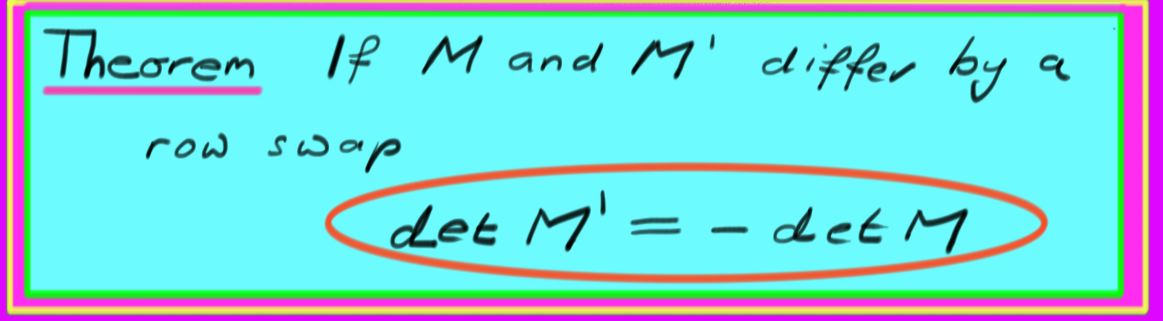
\includegraphics[scale=.3]{\elemMatDetPath/row_swap_theorem.jpg}
\end{center}
\caption{Remember what row swap does to determinants!}
\end{figure}

\section{Elementary Matrices and Determinants}\index{Elementary matrix}

In chapter~\ref{systems} we found
the matrices that perform the  row operations involved in Gaussian elimination; we called them elementary matrices.

As a reminder, for any matrix $M$, and a matrix $M'$ equal to~$M$ after a row operation, multiplying by an elementary matrix $E$ gave $M'=EM$.

\Videoscriptlink{elementary_matrices_determinant_explanation.mp4}{Elementary Matrices}{scripts_elementary_matrices_explanation}

We now examine what the elementary matrices to do determinants.

\subsection{Row Swap}
Our first elementary matrix   swaps  rows $i$ and~$j$ when it is applied to  a matrix $M$. 
Explicitly, 
let $R^1$ through $R^n$ denote the rows  of $M$, and let $M'$ be the matrix $M$ with rows $i$ and $j$ swapped.  Then $M$ and $M'$ can be regarded as a block matrices (where the blocks are rows);
\[
M=\ccolvec{\vdots \\ R^i \\ \vdots \\ R^j \\ \vdots} \text{ and }
M'=\ccolvec{\vdots \\ R^j \\ \vdots \\ R^i \\ \vdots}.
\]
Then notice that
\[
M'=\ccolvec{\\ \vdots \\ R^j \\ \vdots \\ R^i \\ \vdots\\ \\  }= 
\begin{pmatrix}
1 & & & & & & \\
& \ddots & & & & & \\
& & 0 & & 1 & & \\
& & & \ddots & & & \\
& & 1 & & 0 & & \\
& & & & & \ddots & \\
& & & & & & 1 \\
\end{pmatrix}
\ccolvec{\\ \vdots \\ R^i \\ \vdots \\ R^j \\ \vdots \\ \\  }.
\]
The matrix 
\[
\begin{pmatrix}
1 & & & & & & \\
& \ddots & & & & & \\
& & 0 & & 1 & & \\
& & & \ddots & & & \\
& & 1 & & 0 & & \\
& & & & & \ddots & \\
& & & & & & 1 \\
\end{pmatrix}=:E^i_j
\]
is just the identity matrix with rows $i$ and $j$ swapped.  \hypertarget{elem_matrix_row_swap}The matrix $E^i_j$ is an \emph{elementary matrix}\index{Elementary matrix!swapping rows} and
\[
M'=E^i_jM\, .
\]
Because $\det I=1$ and swapping a pair of rows changes the sign of the determinant, we have found that 
\[
\det E^i_j = -1\, .
\]


%\begin{center}
%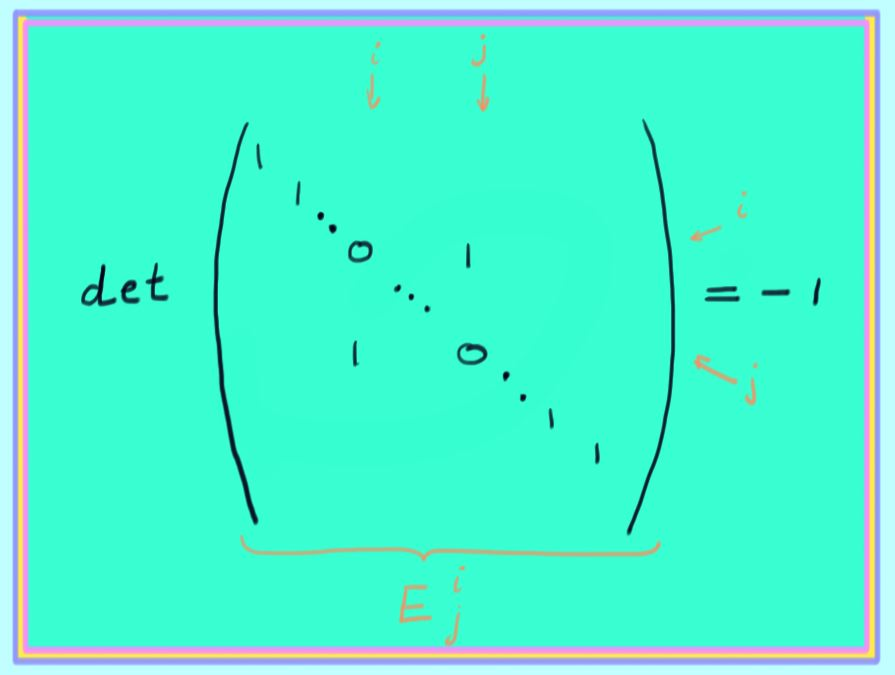
\includegraphics[scale=.25]{\elemMatDetIIPath/detEij.jpg}
%\end{center}

Now we know that swapping a pair of rows flips the sign of the determinant so $\det M'=-det M$.
But $\det E_j^i=-1$ and $M'=E^i_j M$ so 
\[
\det E^i_j M = \det E^i_j \, \det M\, .
\]
This result hints at a general rule for determinants of products of matrices. 
%Stare at it again before reading the next Lecture:
%\begin{center}
%
\includegraphics[scale=.2]{\elemMatDetPath/detEM=detEdetM.jpg}
%\end{center}


%\section*{References}
%Hefferon, Chapter Four, Section I.1 and I.3
%\\
%Beezer, Chapter D, Section DM, Subsection EM
%\\
%Beezer, Chapter D, Section PDM
%\\
%Wikipedia:
%\begin{itemize}
%\item \href{http://en.wikipedia.org/wiki/Determinant}{Determinant}
%\item \href{http://en.wikipedia.org/wiki/Permutation}{Permutation}
%\item \href{http://en.wikipedia.org/wiki/Elementary_matrix}{Elementary Matrix}
%\end{itemize}
%

%\section{Review Problems}
%



\begin{enumerate}
\item \label{det33} Let $M=\begin{pmatrix}
m^1_1 & m^1_2 & m^1_3\\
m^2_1 & m^2_2 & m^2_3\\
m^3_1 & m^3_2 & m^3_3\\
\end{pmatrix}$.  Use row operations to put $M$ into \emph{row echelon form}.  For simplicity, assume that $m_1^1\neq 0 \neq m^1_1m^2_2-m^2_1m^1_2$.

Prove that $M$ is non-singular if and only if:
\[
m^1_1m^2_2m^3_3 
- m^1_1m^2_3m^3_2 
+ m^1_2m^2_3m^3_1 
- m^1_2m^2_1m^3_3 
+ m^1_3m^2_1m^3_2
- m^1_3m^2_2m^3_1
\neq 0
\]

\phantomnewpage

\item 
\begin{enumerate}
\item What does the matrix $E^1_2=\begin{pmatrix}
0 & 1 \\
1 & 0
\end{pmatrix}$ do to $M=\begin{pmatrix}
a & b \\
d & c
\end{pmatrix}$ under left multiplication?  What about right multiplication?
\item Find elementary matrices $R^1(\lambda)$ and $R^2(\lambda)$ that respectively multiply rows $1$ and $2$ of $M$ by $\lambda$ but otherwise leave $M$ the same under left multiplication.
\item Find a matrix $S^1_2(\lambda)$ that adds a multiple $\lambda$ of row $2$ to row $1$ under left multiplication.
\end{enumerate}

\phantomnewpage

\item Let $M$ be a matrix and $S^i_jM$ the same matrix with rows \(i\) and \(j\) switched.  Explain every line of the 
\hyperlink{rowswap}{series of equations} proving that $\det M = -\det (S^i_jM)$.

\phantomnewpage

%\item \label{prob_inversion_number} This problem is a ``hands-on'' look at why \hyperlink{permutation_parity}{the property} describing the parity of permutations is true.
%
%\hypertarget{inversion_number}{The \emph{inversion number}}\index{Permutation!Inversion number} of a permutation $\sigma$ is the number of pairs $i<j$ such that $\sigma(i)>\sigma(j)$; it's the number of ``numbers that appear left of smaller numbers'' in the permutation.  For example, for the permutation $\rho = [4,2,3,1]$, the inversion number is $5$. The number $4$ comes before $2,3,$ and $1$, and $2$ and $3$ both come before $1$.
%
%Given a permutation $\sigma$, we can make a new permutation $\tau_{i,j} \sigma$ by exchanging the $i$th and $j$th entries of $\sigma$.
%
%\begin{enumerate}
%\item What is the inversion number of the permutation \(\mu=[1,2,4,3]\) that exchanges 4 and 3 and leaves everything else alone? Is it an even or an odd permutation?
%
%\item What is the inversion number of the permutation \(\rho=[4,2,3,1]\) that exchanges 1 and 4 and leaves everything else alone? Is it an even or an odd permutation?
%
%\item What is the inversion number of the permutation \(\tau_{1,3} \mu\)? Compare the parity\footnote{The \emph{parity} of an integer refers to whether the integer is even or odd. Here the parity of a permutation $\mu$ refers to the parity of its inversion number.} of \(\mu\) to the parity of \(\tau_{1,3} \mu.\)
%
%\item What is the inversion number of the permutation \(\tau_{2,4} \rho\)? Compare the parity of \(\rho\) to the parity of \(\tau_{2,4} \rho.\)
%
%\item What is the inversion number of the permutation \(\tau_{3,4} \rho\)? Compare the parity of \(\rho\) to the parity of \(\tau_{3,4} \rho.\)
%\end{enumerate}
%
%\videoscriptlink{elementary_matrices_determinant_hint.mp4}{Problem~\ref{prob_inversion_number} hints}{scripts_elementary_matrices_determinants_hint}

\phantomnewpage

%\item \label{problem_permutation} (Extra credit) Here we will examine a (very) small set of the general properties about permutations and their applications. In particular, we will show that one way to compute the sign of a permutation is by finding the \hyperlink{inversion_number}{inversion number} $N$ of $\sigma$ and we have
%\[
%\sgn(\sigma) = (-1)^N.
%\]
%
%For this problem, let $\mu = [1,2,4,3]$.
%
%\begin{enumerate}
%\item Show that every permutation $\sigma$ can be sorted by only taking simple (adjacent) transpositions\index{Permutation!Simple transposition} $s_i$ where $s_i$ interchanges the numbers in position $i$ and $i+1$ of a permutation $\sigma$ (in our other notation $s_i = \tau_{i,i+1}$). For example $s_2 \mu = [1, 4, 2, 3]$, and to sort $\mu$ we have $s_3 \mu = [1, 2, 3, 4]$.
%
%\item \label{prob_part_relations} We can compose simple transpositions together to represent a permutation (note that the sequence of compositions is not unique), and these are associative, we have an identity (the trivial permutation where the list is in order or we do nothing on our list), and we have an inverse since it is clear that $s_i s_i \sigma = \sigma$. Thus permutations of $[n]$ under composition are an example of a \hyperref[groups]{group}. However note that not all simple transpositions commute with each other since
%\begin{align*}
%s_1 s_2 [1, 2, 3] & = s_1 [1, 3, 2] = [3, 1, 2]
%\\ s_2 s_1 [1, 2, 3] & = s_2 [2, 1, 3] = [2, 3, 1]
%\end{align*}
%(you will prove here when simple transpositions commute). When we consider our initial permutation to be the trivial permutation $e = [1, 2, \dotsc, n]$, we do not write it; for example $s_i \equiv s_i e$ and $\mu = s_3 \equiv s_3 e$. This is analogous to not writing 1 when multiplying. Show that $s_i s_i = e$ (in shorthand $s_i^2 = e$), $s_{i+1} s_i s_{i+1} = s_i s_{i+1} s_i$ for all $i$, and $s_i$ and $s_j$ commute for all $|i - j| \geq 2$.
%
%\item Show that every way of expressing $\sigma$ can be obtained from using the relations proved in part~\ref{prob_part_relations}. In other words, show that for any expression $w$ of simple transpositions representing the trivial permutation $e$, using the proved relations.
%
%\emph{Hint: Use induction on $n$. For the induction step, follow the path of the $(n+1)$-th strand by looking at $s_n s_{n-1} \cdots s_k s_{k\pm1} \cdots s_n$ and argue why you can write this as a subexpression for any expression of $e$. Consider using diagrams of these paths to help.}
%
%\item The simple transpositions \hyperlink{action}{acts on} an $n$-dimensional vector space $V$ by $s_i v = E^i_{i+1} v$ (where $E^i_j$ is \hyperlink{elem_matrix_row_swap}{an elementary matrix}) for all vectors $v \in V$. Therefore we can just represent a permutation $\sigma$ as the matrix $M_{\sigma}$\footnote{Often people will just use $\sigma$ for the matrix when the context is clear.}, and we have $\det(M_{s_i}) = \det(E^i_{i+1}) = -1$. Thus prove that $\det(M_{\sigma}) = (-1)^N$ where $N$ is a number of simple transpositions needed to represent $\sigma$ as a permutation. You can assume that $M_{s_i s_j} = M_{s_i} M_{s_j}$ (it is not hard to prove) and that $\det(A B) = \det(A) \det(B)$ \hyperref[detmultiplicative]{from Chapter~\ref*{elementarydeterminantsII}}.
%
%\emph{Hint: You to make sure $\det(M_{\sigma})$ is well-defined since there are infinite ways to represent $\sigma$ as simple transpositions.}
%
%\item Show that $s_{i+1} s_i s_{i+1} = \tau_{i, i+2}$, and so give one way of writing $\tau_{i, j}$ in terms of simple transpositions? Is $\tau_{i,j}$ an even or an odd permutation? What is $\det(M_{\tau_{i,j}})$? What is the inversion number of $\tau_{i,j}$?
%
%\item The minimal number of simple transpositions needed to express $\sigma$ is called the \emph{length}\index{Permutation!Length} of $\sigma$; for example the length of $\mu$ is 1 since $\mu = s_3$. Show that the length of $\sigma$ is equal to the inversion number of $\sigma$.
%
%\emph{Hint: Find an procedure which gives you a new permutation $\sigma^{\prime}$ where $\sigma = s_i \sigma^{\prime}$ for some $i$ and the inversion number for $\sigma^{\prime}$ is 1 less than the inversion number for $\sigma$.}
%
%\item Show that $(-1)^N = \sgn(\sigma) = \det(M_{\sigma})$, where $\sigma$ is a permutation with $N$ inversions. Note that this immediately implies that $\sgn(\sigma \rho) = \sgn(\sigma) \sgn(\rho)$ for any permutations $\sigma$ and $\rho$.
%\end{enumerate}

\item Let $M'$ be the matrix obtained from $M$ by swapping two columns $i$ and $j$. Show that $\det M'=-\det M $.

\item The scalar triple product of three vectors $u,v,w$ from $\Re^3$ is $u\cdot(v\times w)$. Show that this product is the same as the determinant of the matrix whose columns are $u,v,w$ (in that order). What happens to the scalar triple product when the factors are permuted? 

\item Show that if $M$ is a $3\times 3$ matrix whose third row is a sum of multiples of the other rows ($R_3=aR_2+bR_1$) then $\det M=0$. Show that the same is true if one of the columns is a sum of multiples of the others. 

\end{enumerate}

\phantomnewpage

%\section{\elemMatDetIITitle}\label{elementarydeterminantsII}

%In section~\ref{elementarydeterminants}, we saw the definition of the determinant and derived an elementary matrix that exchanges two rows of a matrix.  

\subsection{Row  Multiplication}
The next row operation is multiplying a row by a scalar.
Consider \[M=\ccolvec{R^1 \\ \vdots \\ R^n }\, ,\] where $R^i$ are row vectors.  Let $R^i(\lambda)$ be the identity matrix, with the $i$th diagonal entry replaced by $\lambda$, not to be confused with the row vectors. {\itshape I.e.},
\[
R^i(\lambda)=
\begin{pmatrix}
1 & & & & \\
  & \ddots & & & \\
  & & \lambda & & \\
  & & & \ddots & \\
  & & & & 1 \\
\end{pmatrix}
\, .\]
Then:
\[
M'=R^i(\lambda)M=\ccolvec{R^1 \\ \vdots \\ \lambda R^i \\ \vdots \\ R^n }\, ,
\]
equals $M$ with one row multiplied by~$\lambda$.

What effect does multiplication by the elementary matrix $R^i(\lambda)$ have on the determinant?

\begin{eqnarray*}
\det M' & = & \sum_{\sigma} \text{sgn}(\sigma) m^1_{\sigma(1)}\cdots \lambda m^i_{\sigma(i)} \cdots m^n_{\sigma(n)} \\
& = & \lambda \sum_{\sigma} \text{sgn}(\sigma) m^1_{\sigma(1)}\cdots m^i_{\sigma(i)} \cdots m^n_{\sigma(n)} \\
& = & \lambda \det M
\end{eqnarray*}
Thus, multiplying a row by $\lambda$ multiplies the determinant by $\lambda$.
{\itshape I.e.,} \[\det R^i(\lambda) M = \lambda \det M\, .\]


\begin{figure}
\begin{center}
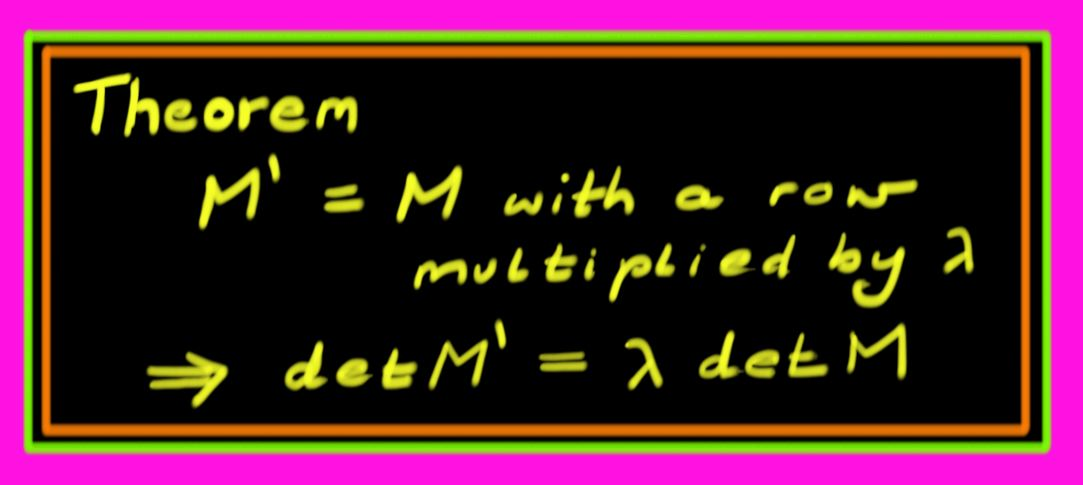
\includegraphics[scale=.27]{\elemMatDetIIPath/row_mult_thm.jpg}
\end{center}
\caption{Rescaling a row rescales the determinant.}
\end{figure}


Since $R^i(\lambda)$ is just the identity matrix with a single row multiplied by $\lambda$, then by the above rule, the determinant of $R^i(\lambda)$ is $\lambda$.  Thus

\[
\det R^i(\lambda) = \det \begin{pmatrix}
1 & & & & \\
  & \ddots & & & \\
  & & \lambda & & \\
  & & & \ddots & \\
  & & & & 1 \\
\end{pmatrix} = \lambda\, ,
\]
and once again we have a product of determinants formula
\[
\det \left( R^i(\lambda) M \right) = \det\left( R^i(\lambda) \right)\det M.
\]

\subsection{Row Addition}
The final row operation is adding $\mu R^j$ to $R^i$.  This is done with the elementary matrix~$S^i_j(\mu)$, which is an identity matrix but with an additional  $\mu$ in the $i,j$ position;

\[
S^i_j(\mu) = \begin{pmatrix}
1 & 	& 	& 	& & & 	\\
  & \ddots & 	&	& & &	\\
  & 	& 1 	& 	& \mu & &	\\
  & 	& 	& \ddots & & &	\\
  & 	& 	& 	& 1 & & 	\\
  & 	& 	& 	& 	& \ddots & 	\\
  & 	& 	& 	& 	& 	 & 1	\\
\end{pmatrix}\, .
\]
Then multiplying $M$ by $S^i_j(\mu)$  performs a row addition;

\[
\begin{pmatrix}
1 & 	& 	& 	& & & 	\\
  & \ddots & 	&	& & &	\\
  & 	& 1 	& 	& \mu & &	\\
  & 	& 	& \ddots & & &	\\
  & 	& 	& 	& 1 & & 	\\
  & 	& 	& 	& 	& \ddots & 	\\
  & 	& 	& 	& 	& 	 & 1	\\
\end{pmatrix}\ccolvec{\\ \vdots \\ R^i \\ \vdots \\ R^j \\ \vdots\\ \\}
=
\ccolvec{\\ \vdots \\ R^i +\mu R^j \\ \vdots \\ R^j \\ \vdots\\ \\ }\, .
\]
What is the effect of multiplying by $S^i_j(\mu)$ on the determinant?  Let $M'=S^i_j(\mu)M$, and let $M''$ be the matrix $M$ but with $R^i$ replaced by $R^j$
Then

\begin{eqnarray*}
\det M' & = & \sum_{\sigma} \text{sgn}(\sigma) m^1_{\sigma(1)}\cdots (m^i_{\sigma(i)}+ \mu m^j_{\sigma(i)}) \cdots m^n_{\sigma(n)} \\
& = & \sum_{\sigma} \text{sgn}(\sigma) m^1_{\sigma(1)}\cdots m^i_{\sigma(i)} \cdots m^n_{\sigma(n)} \\
&   & \qquad + \sum_{\sigma} \text{sgn}(\sigma) m^1_{\sigma(1)}\cdots \mu m^j_{\sigma(j)} \cdots m^j_{\sigma(j)} \cdots m^n_{\sigma(n)} \\
& = & \det M + \mu \det M''
\end{eqnarray*}
Since $M''$ has two identical rows, its determinant is $0$ so
\[
\det M' = \det M,
\]
when $M'$ is obtained from $M$ by adding $\mu$ times row~$j$ to row~$i$.

%\href{\webworkurl ReadingHomework13/1/}{Reading homework: problem 13.1}
\Reading{Determinants}{3}

\noindent
We also have learnt that
\[\det \left( S^i_j(\mu)M \right) = \det M\, .\]
Notice that if $M$ is the identity matrix, then we have \[\det S^i_j(\mu) = \det (S^i_j(\mu)I) = \det I = 1\, .\]



\begin{figure}
\begin{center}
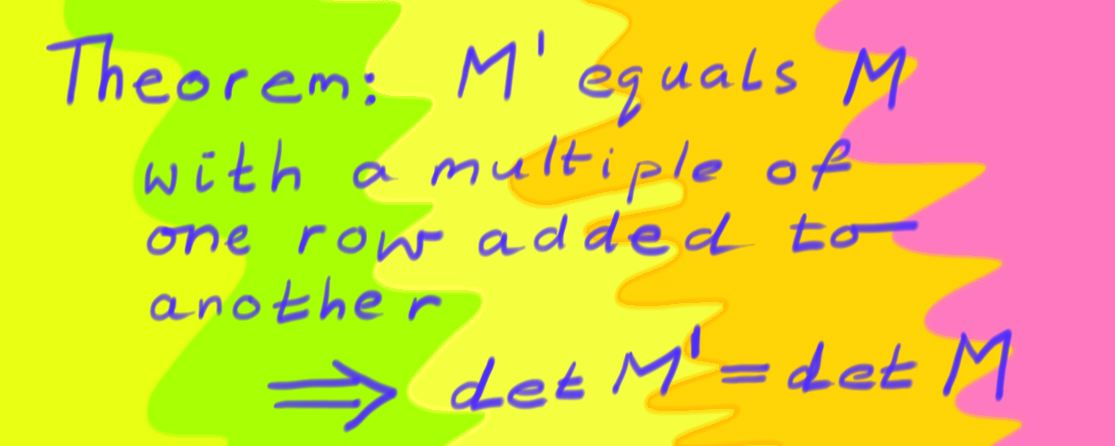
\includegraphics[scale=.27]{\elemMatDetIIPath/row_addition_thm.jpg}
\end{center}
\caption{Adding one row to another leaves the determinant unchanged.}
\end{figure}

\subsection{Determinant of Products}
In summary, the elementary matrices for each of the row operations obey

\[
\begin{array}{cccc}
E^i_j &=& I \text{ with rows $i,j$ swapped;} &\det E^i_j=-1 \\[3mm]
R^i(\lambda) &=& I \text{ with $\lambda$ in position $i,i$;} 
	&\det R^i(\lambda)=\lambda \\[3mm]
S^i_j(\mu) &=& I \text{ with $\mu$ in position $i,j$;} 
	&\det S^i_j(\mu)=1 \\[3mm]
\end{array}
\]
\Videoscriptlink{elementary_matrices_and_determinants_ii_dets.mp4}{Elementary Determinants}{scripts_elementary_matrices_determinants_ii_dets}

Moreover  we found a useful formula for determinants of products:

\begin{theorem}
If $E$ is \emph{ any} of the elementary matrices $E^i_j, R^i(\lambda), S^i_j(\mu)$, then $\det(EM)=\det E \det M$.
\end{theorem}


%\begin{center}
%\hspace{3mm}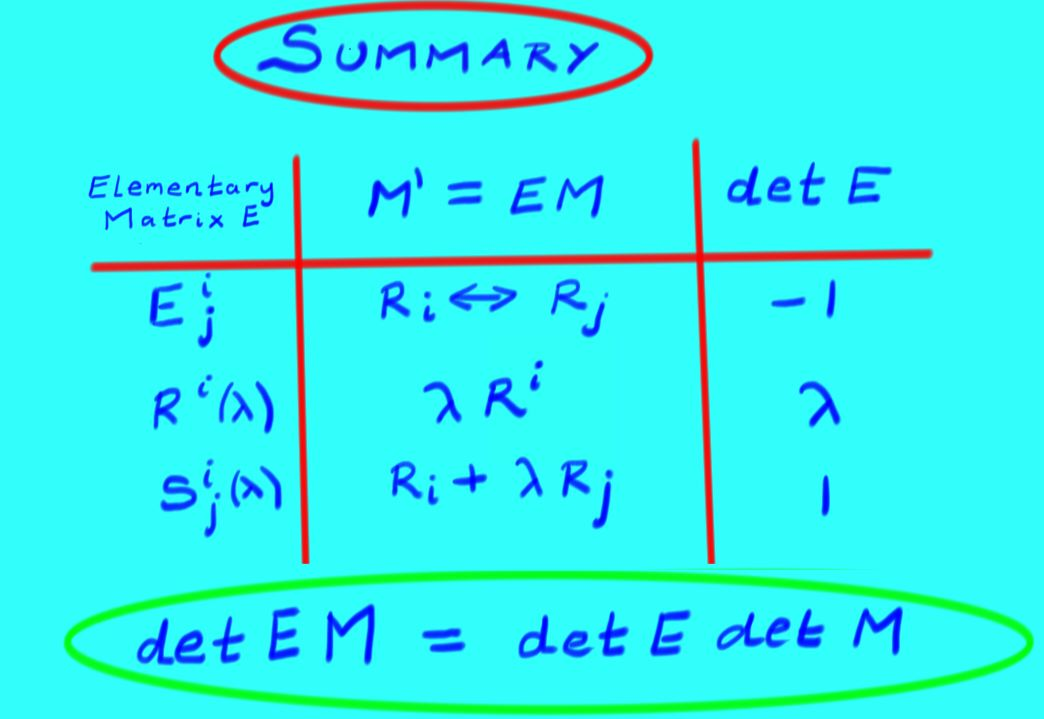
\includegraphics[scale=.27]{\elemMatDetIIPath/summary.jpg}
%\end{center}


We have seen that any matrix $M$ can be put into reduced row echelon form via a sequence of row operations, and we have seen that any row operation can be achieved via left matrix multiplication by an elementary matrix.  Suppose that $\rref(M)$ is the reduced row echelon form of $M$.  Then \[\rref(M)=E_1E_2\cdots E_kM\, ,\] where each $E_i$ is an elementary matrix.
We know how to compute determinants of elementary matrices and products thereof, so we ask:

\begin{center}
What is the determinant of a square matrix in reduced row echelon form?  
\end{center}
The answer has two cases:
\begin{enumerate}
\item If $M$ is not invertible, then some row of $\rref(M)$ contains only zeros.  Then we can multiply the zero row by any constant $\lambda$ without changing~$M$; by our previous observation, this scales the determinant of $M$ by $\lambda$.  Thus, if $M$ is not invertible, $\det \rref(M)=\lambda \det \rref(M)$, and so $\det \rref(M)=0$.  

\item Otherwise, every row of $\rref(M)$ has a pivot on the diagonal; since $M$ is square, this means that $\rref(M)$ is the identity matrix.  So if $M$ is invertible, $\det \rref(M)=1$.
\end{enumerate}
Notice that because $\det \rref(M) = \det (E_1E_2\cdots E_kM)$, by the theorem above, \[\det \rref(M)=\det (E_1) \cdots \det (E_k) \det M\, .\]  Since each $E_i$ has non-zero determinant, then $\det \rref(M)=0$ if and only if $\det M=0$.
This establishes an important theorem:


\begin{theorem}
\label{detinvertible}
For any square matrix $M$, $\det M\neq 0$ if and only if $M$ is invertible.
\end{theorem}
Since we know the determinants of the elementary matrices, we can immediately obtain the following:


\Videoscriptlink{elementary_matrices_ii_inverses_determinants.mp4}{Determinants and Inverses}{scripts_elementary_matrices_determinants_ii_inverses}

\begin{figure}
\begin{center}
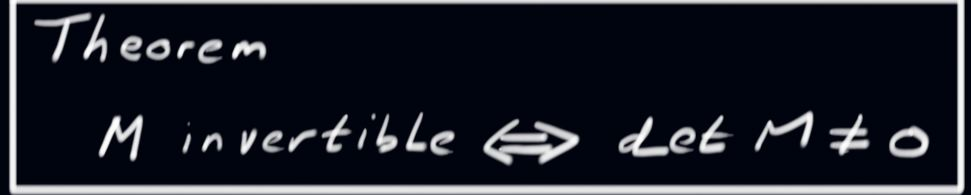
\includegraphics[scale=.27]{\elemMatDetIIPath/theorem_invertible.jpg}
\end{center}
\caption{Determinants measure if a matrix is invertible.}
\end{figure}

\begin{corollary}
Any elementary matrix $E^i_j, R^i(\lambda), S^i_j(\mu)$ is invertible, except for $R^i(0)$.  In fact, the inverse of an elementary matrix is another elementary matrix.
\end{corollary}


To obtain one last important result, suppose that $M$ and $N$ are square $n\times n$ matrices, with reduced row echelon forms such that, for elementary matrices  $E_i$ and $F_i$, \[M=E_1E_2\cdots E_k \, \rref(M)\, ,\] and  \[N=F_1F_2\cdots F_l \, \rref(N)\, .\]  If $\rref(M)$ is the identity matrix ({\itshape i.e.}, $M$ is invertible), then:

\begin{eqnarray*}
\det (MN) & = & \det (E_1E_2\cdots E_k\,  \rref(M) F_1F_2\cdots F_l \, \rref(N) )\\
& = & \det (E_1E_2\cdots E_k I F_1F_2\cdots F_l\,  \rref(N) )\\
& = & \det (E_1) \cdots \det(E_k)\det(I)\det(F_1)\cdots\det(F_l)\det\rref(N)\\
& = & \det(M)\det(N)
\end{eqnarray*}
Otherwise, $M$ is not invertible, and $\det M=0=\det 
\rref(M)$.  Then there exists a row of zeros in $
\rref(M)$, so $R^n(\lambda)
\rref(M)=
\rref(M)$ {\itshape for any~$\lambda$}.  Then:
\begin{eqnarray*}
\det (MN) & = & 
\det (E_1E_2\cdots E_k \, \rref(M) N )\\
& = & 
\det (E_1) \cdots \det(E_k)\det( \rref(M)N)\\
& = & \det (E_1) \cdots \det(E_k)\det( R^n(\lambda) 
\, \rref(M)N)\\
& = & \det (E_1) \cdots \det(E_k)\lambda \det( 
\rref(M)N)\\
& = & \lambda \det (MN)
\end{eqnarray*}
Which implies that $\det (MN)=0=\det M \det N$.

Thus we have shown that for {\itshape any} matrices $M$ and $N$, 
\label{detmultiplicative}
\[
\det (MN) = \det M \det N
\]
This result is {\itshape extremely important}; do not forget it!

\Videoscriptlink{elementary_matrices_determinant_ii_product.mp4}{Alternative proof}{scripts_elementary_matrices_determinants_ii_product}

\begin{figure}
\begin{center}

\includegraphics[scale=.27]{\elemMatDetIIPath/detMN.jpg}
\end{center}
\caption{``The determinant of a product is the product of determinants.''}
\end{figure}





%\href{\webworkurl ReadingHomework13/2/}{Reading homework: problem 13.2}
\Reading{Determinants}{4}

%\section*{References}
%Hefferon, Chapter Four, Section I.1 and I.3
%\\
%Beezer, Chapter D, Section DM, Subsection EM
%\\
%Beezer, Chapter D, Section PDM
%\\
%Wikipedia:
%\begin{itemize}
%\item \href{http://en.wikipedia.org/wiki/Determinant}{Determinant}
%\item \href{http://en.wikipedia.org/wiki/Elementary_matrix}{Elementary Matrix}
%\end{itemize}

\section{Review Problems}

{\bfseries Webwork:} 
\begin{tabular}{|c|c|}
\hline
Reading Problems & 
 \hwrref{Determinants}{1},
 \hwrref{Determinants}{2},
  \hwrref{Determinants}{3},
   \hwrref{Determinants}{4}\\
 $2\times 2$ Determinant & \hwref{Determinants}{7}\\
 Determinants and invertibility & \hwref{Determinants}{8},
 \hwref{Determinants}{9},
 \hwref{Determinants}{10},
 \hwref{Determinants}{11}
 \\\hline
\end{tabular}






\begin{enumerate}
\item \label{det33} Let $M=\begin{pmatrix}
m^1_1 & m^1_2 & m^1_3\\
m^2_1 & m^2_2 & m^2_3\\
m^3_1 & m^3_2 & m^3_3\\
\end{pmatrix}$.  Use row operations to put $M$ into \emph{row echelon form}.  For simplicity, assume that $m_1^1\neq 0 \neq m^1_1m^2_2-m^2_1m^1_2$.

Prove that $M$ is non-singular if and only if:
\[
m^1_1m^2_2m^3_3 
- m^1_1m^2_3m^3_2 
+ m^1_2m^2_3m^3_1 
- m^1_2m^2_1m^3_3 
+ m^1_3m^2_1m^3_2
- m^1_3m^2_2m^3_1
\neq 0
\]

\phantomnewpage

\item 
\begin{enumerate}
\item What does the matrix $E^1_2=\begin{pmatrix}
0 & 1 \\
1 & 0
\end{pmatrix}$ do to $M=\begin{pmatrix}
a & b \\
d & c
\end{pmatrix}$ under left multiplication?  What about right multiplication?
\item Find elementary matrices $R^1(\lambda)$ and $R^2(\lambda)$ that respectively multiply rows $1$ and $2$ of $M$ by $\lambda$ but otherwise leave $M$ the same under left multiplication.
\item Find a matrix $S^1_2(\lambda)$ that adds a multiple $\lambda$ of row $2$ to row $1$ under left multiplication.
\end{enumerate}

\phantomnewpage

\item Let $M$ be a matrix and $S^i_jM$ the same matrix with rows \(i\) and \(j\) switched.  Explain every line of the 
\hyperlink{rowswap}{series of equations} proving that $\det M = -\det (S^i_jM)$.

\phantomnewpage

%\item \label{prob_inversion_number} This problem is a ``hands-on'' look at why \hyperlink{permutation_parity}{the property} describing the parity of permutations is true.
%
%\hypertarget{inversion_number}{The \emph{inversion number}}\index{Permutation!Inversion number} of a permutation $\sigma$ is the number of pairs $i<j$ such that $\sigma(i)>\sigma(j)$; it's the number of ``numbers that appear left of smaller numbers'' in the permutation.  For example, for the permutation $\rho = [4,2,3,1]$, the inversion number is $5$. The number $4$ comes before $2,3,$ and $1$, and $2$ and $3$ both come before $1$.
%
%Given a permutation $\sigma$, we can make a new permutation $\tau_{i,j} \sigma$ by exchanging the $i$th and $j$th entries of $\sigma$.
%
%\begin{enumerate}
%\item What is the inversion number of the permutation \(\mu=[1,2,4,3]\) that exchanges 4 and 3 and leaves everything else alone? Is it an even or an odd permutation?
%
%\item What is the inversion number of the permutation \(\rho=[4,2,3,1]\) that exchanges 1 and 4 and leaves everything else alone? Is it an even or an odd permutation?
%
%\item What is the inversion number of the permutation \(\tau_{1,3} \mu\)? Compare the parity\footnote{The \emph{parity} of an integer refers to whether the integer is even or odd. Here the parity of a permutation $\mu$ refers to the parity of its inversion number.} of \(\mu\) to the parity of \(\tau_{1,3} \mu.\)
%
%\item What is the inversion number of the permutation \(\tau_{2,4} \rho\)? Compare the parity of \(\rho\) to the parity of \(\tau_{2,4} \rho.\)
%
%\item What is the inversion number of the permutation \(\tau_{3,4} \rho\)? Compare the parity of \(\rho\) to the parity of \(\tau_{3,4} \rho.\)
%\end{enumerate}
%
%\videoscriptlink{elementary_matrices_determinant_hint.mp4}{Problem~\ref{prob_inversion_number} hints}{scripts_elementary_matrices_determinants_hint}

\phantomnewpage

%\item \label{problem_permutation} (Extra credit) Here we will examine a (very) small set of the general properties about permutations and their applications. In particular, we will show that one way to compute the sign of a permutation is by finding the \hyperlink{inversion_number}{inversion number} $N$ of $\sigma$ and we have
%\[
%\sgn(\sigma) = (-1)^N.
%\]
%
%For this problem, let $\mu = [1,2,4,3]$.
%
%\begin{enumerate}
%\item Show that every permutation $\sigma$ can be sorted by only taking simple (adjacent) transpositions\index{Permutation!Simple transposition} $s_i$ where $s_i$ interchanges the numbers in position $i$ and $i+1$ of a permutation $\sigma$ (in our other notation $s_i = \tau_{i,i+1}$). For example $s_2 \mu = [1, 4, 2, 3]$, and to sort $\mu$ we have $s_3 \mu = [1, 2, 3, 4]$.
%
%\item \label{prob_part_relations} We can compose simple transpositions together to represent a permutation (note that the sequence of compositions is not unique), and these are associative, we have an identity (the trivial permutation where the list is in order or we do nothing on our list), and we have an inverse since it is clear that $s_i s_i \sigma = \sigma$. Thus permutations of $[n]$ under composition are an example of a \hyperref[groups]{group}. However note that not all simple transpositions commute with each other since
%\begin{align*}
%s_1 s_2 [1, 2, 3] & = s_1 [1, 3, 2] = [3, 1, 2]
%\\ s_2 s_1 [1, 2, 3] & = s_2 [2, 1, 3] = [2, 3, 1]
%\end{align*}
%(you will prove here when simple transpositions commute). When we consider our initial permutation to be the trivial permutation $e = [1, 2, \dotsc, n]$, we do not write it; for example $s_i \equiv s_i e$ and $\mu = s_3 \equiv s_3 e$. This is analogous to not writing 1 when multiplying. Show that $s_i s_i = e$ (in shorthand $s_i^2 = e$), $s_{i+1} s_i s_{i+1} = s_i s_{i+1} s_i$ for all $i$, and $s_i$ and $s_j$ commute for all $|i - j| \geq 2$.
%
%\item Show that every way of expressing $\sigma$ can be obtained from using the relations proved in part~\ref{prob_part_relations}. In other words, show that for any expression $w$ of simple transpositions representing the trivial permutation $e$, using the proved relations.
%
%\emph{Hint: Use induction on $n$. For the induction step, follow the path of the $(n+1)$-th strand by looking at $s_n s_{n-1} \cdots s_k s_{k\pm1} \cdots s_n$ and argue why you can write this as a subexpression for any expression of $e$. Consider using diagrams of these paths to help.}
%
%\item The simple transpositions \hyperlink{action}{acts on} an $n$-dimensional vector space $V$ by $s_i v = E^i_{i+1} v$ (where $E^i_j$ is \hyperlink{elem_matrix_row_swap}{an elementary matrix}) for all vectors $v \in V$. Therefore we can just represent a permutation $\sigma$ as the matrix $M_{\sigma}$\footnote{Often people will just use $\sigma$ for the matrix when the context is clear.}, and we have $\det(M_{s_i}) = \det(E^i_{i+1}) = -1$. Thus prove that $\det(M_{\sigma}) = (-1)^N$ where $N$ is a number of simple transpositions needed to represent $\sigma$ as a permutation. You can assume that $M_{s_i s_j} = M_{s_i} M_{s_j}$ (it is not hard to prove) and that $\det(A B) = \det(A) \det(B)$ \hyperref[detmultiplicative]{from Chapter~\ref*{elementarydeterminantsII}}.
%
%\emph{Hint: You to make sure $\det(M_{\sigma})$ is well-defined since there are infinite ways to represent $\sigma$ as simple transpositions.}
%
%\item Show that $s_{i+1} s_i s_{i+1} = \tau_{i, i+2}$, and so give one way of writing $\tau_{i, j}$ in terms of simple transpositions? Is $\tau_{i,j}$ an even or an odd permutation? What is $\det(M_{\tau_{i,j}})$? What is the inversion number of $\tau_{i,j}$?
%
%\item The minimal number of simple transpositions needed to express $\sigma$ is called the \emph{length}\index{Permutation!Length} of $\sigma$; for example the length of $\mu$ is 1 since $\mu = s_3$. Show that the length of $\sigma$ is equal to the inversion number of $\sigma$.
%
%\emph{Hint: Find an procedure which gives you a new permutation $\sigma^{\prime}$ where $\sigma = s_i \sigma^{\prime}$ for some $i$ and the inversion number for $\sigma^{\prime}$ is 1 less than the inversion number for $\sigma$.}
%
%\item Show that $(-1)^N = \sgn(\sigma) = \det(M_{\sigma})$, where $\sigma$ is a permutation with $N$ inversions. Note that this immediately implies that $\sgn(\sigma \rho) = \sgn(\sigma) \sgn(\rho)$ for any permutations $\sigma$ and $\rho$.
%\end{enumerate}

\item Let $M'$ be the matrix obtained from $M$ by swapping two columns $i$ and $j$. Show that $\det M'=-\det M $.

\item The scalar triple product of three vectors $u,v,w$ from $\Re^3$ is $u\cdot(v\times w)$. Show that this product is the same as the determinant of the matrix whose columns are $u,v,w$ (in that order). What happens to the scalar triple product when the factors are permuted? 

\item Show that if $M$ is a $3\times 3$ matrix whose third row is a sum of multiples of the other rows ($R_3=aR_2+bR_1$) then $\det M=0$. Show that the same is true if one of the columns is a sum of multiples of the others. 

\end{enumerate}

\phantomnewpage

\newpage

\section{\propDetTitle}

%In section~\ref{elementarydeterminantsII} we \hyperref[detinvertible]{showed} 
We now know that the determinant of a matrix is non-zero if and only if that matrix is invertible.  We also 
know 
%\hyperref[detmultiplicative]{showed} 
that the determinant is a \emph{multiplicative} function\index{Multiplicative function}, in the sense that $\det (MN)=\det M \det N$.  Now we will devise some methods for calculating the determinant.

Recall that:
\[
\det M = \sum_{\sigma} \text{sgn}(\sigma) m^1_{\sigma(1)}m^2_{\sigma(2)}\cdots m^n_{\sigma(n)}.
\]

A \emph{minor}\index{Minor} of an $n\times n$ matrix $M$ is the determinant of any square matrix obtained from $M$ by deleting one row and one column.  In particular, any entry $m^i_j$ of a square matrix~$M$ is associated to a minor obtained by deleting the $i$th row and $j$th column of~$M$.

It is possible to write the determinant of a matrix in terms of  its minors\index{Expansion by minors} as follows:

\begin{eqnarray*}
\det M &=& \sum_{\sigma} \text{sgn}(\sigma)\, m^1_{\sigma(1)}m^2_{\sigma(2)}\cdots m^n_{\sigma(n)} \\
&=& m^1_1\, \sum_{\slashed{\sigma}^1} \text{sgn}(\slashed{\sigma}^1)\, m^2_{\slashed{\sigma}^1(2)}\cdots m^n_{\slashed{\sigma}^1(n)} \\
& +&  m^1_2\, \sum_{\slashed{\sigma}^2} \text{sgn}(\slashed{\sigma}^2)\, m^2_{\slashed{\sigma}^2(1)}
m^3_{\slashed{\sigma}^2(3)}\cdots m^n_{\slashed{\sigma}^2(n)} \\
& +&  m^1_3\,  \sum_{\slashed{\sigma}^3} \text{sgn}(\slashed{\sigma}^3)\, m^2_{\slashed{\sigma}^3(1)}m^3_{\slashed{\sigma}^3(2)}m^4_{\slashed{\sigma}^3(4)}\cdots m^n_{\slashed{\sigma}^3(n)}\\ &+& \cdots
\end{eqnarray*}
Here the symbols $\slashed{\sigma}^k$ 
refers to the permutation $\sigma$ with the input $k$ removed.
The summand on  the $j$'th line of the above formula looks like the determinant of the minor obtained by removing the first  and $j$'th column of $M$. However we still need to  replace sum of $\slashed{\sigma}^j$ by a sum over permutations of  column numbers of the matrix entries of this minor. This costs a minus sign whenever $j-1$ is odd.
%refer to permutations of $n-1$ objects.  What we're doing here is collecting up all of the terms of the original sum that contain the first 
%row entry $m^1_j$ for each column number $j$.  Each term in that collection is associated to a permutation sending $1\rightarrow j$.  The remainder of any such permutation maps the set $\{2, \ldots, n \}\rightarrow \{1, \ldots, j-1, j+1, \ldots, n \}$.  We call this partial permutation $\hat{\sigma}=\begin{bmatrix} \sigma(2) & \cdots & \sigma(n) \end{bmatrix}$.
%The last issue is that the permutation $\hat{\sigma}$ may not have the same sign as $\sigma$.  From previous homework, we know that a permutation has the same parity as its inversion number.  Removing $1\rightarrow j$ from a permutation  reduces the inversion number by the number of elements right of $j$ that are less than~$j$.  Since $j$ comes first in the permutation $\begin{bmatrix}j & \sigma(2) & \cdots & \sigma(n) \end{bmatrix}$, the inversion number of $\hat{\sigma}$ is reduced by $j-1$.  Then the sign of~$\sigma$ differs from the sign of~$\hat{\sigma}$ if $\sigma$ sends $1$ to an even number.
In other words, to expand by minors we pick an entry $m^1_j$ of the first row, then add $(-1)^{j-1}$ times the determinant of the matrix with row $i$ and column~$j$ deleted. An example will probably help:

\begin{example}
Let's compute the determinant of 
\[M=\begin{pmatrix}
1 & 2 & 3 \\
4 & 5 & 6 \\
7 & 8 & 9 \\
\end{pmatrix}\] using expansion by minors:

\begin{eqnarray*}
\det M & = & 1\det \begin{pmatrix}
5 & 6 \\
8 & 9 \\
\end{pmatrix}
-2 \det \begin{pmatrix}
4 & 6 \\
7 & 9 \\
\end{pmatrix}
+3 \det \begin{pmatrix}
4 & 5 \\
7 & 8 \\
\end{pmatrix} \\
& = & 1(5\cdot 9- 8\cdot 6) -2 (4\cdot 9- 7\cdot 6) + 3 (4\cdot 8- 7\cdot 5) \\[1mm]
& = & 0 \\
\end{eqnarray*}
Here, $M^{-1}$ does not exist because\footnote{A fun exercise is to compute the determinant of a $4\times 4$ matrix filled in order, from left to right,  with the numbers $1,2,3,\ldots, 16$. What do you observe? Try the same for a $5\times 5$ matrix with $1,2,3,\ldots, 25$. Is there a pattern? Can you explain it?} $\det M=0.$
\end{example}


\begin{example}
Sometimes the entries of a matrix allow us to simplify the calculation of the determinant.  Take $N= \begin{pmatrix}
1 & 2 & 3 \\
4 & 0 & 0 \\
7 & 8 & 9 \\
\end{pmatrix}$.  Notice that the second row has many zeros; then we can switch the first and second rows of $N$ before expanding in minors to get:

\begin{eqnarray*}
\det \begin{pmatrix}
1 & 2 & 3 \\
4 & 0 & 0 \\
7 & 8 & 9 \\
\end{pmatrix} & = & -\det \begin{pmatrix}
4 & 0 & 0 \\
1 & 2 & 3 \\
7 & 8 & 9 \\
\end{pmatrix}\\
&=& -4 \det \begin{pmatrix}
2 & 3 \\
8 & 9 \\
\end{pmatrix} \\
&=& 24
\end{eqnarray*}
\end{example}
 
\Videoscriptlink{properties_of_determinant_practice.mp4}{Example}{video_properties_of_determinant_practice}

Since we know how the determinant of a matrix changes when you perform row operations, it is often very beneficial to perform row
operations before computing the determinant by brute force.

\begin{example}
\begin{eqnarray*}
\det\begin{pmatrix}
1 & 2 & 3 \\
4 & 5 & 6 \\
7 & 8 & 9 \\
\end{pmatrix}
=
\det\begin{pmatrix}
1 & 2 & 3 \\
3 & 3 & 3 \\
6 & 6 & 6 \\
\end{pmatrix}
=
\det\begin{pmatrix}
1 & 2 & 3 \\
3 & 3 & 3 \\
0 & 0 & 0 \\
\end{pmatrix}=0\, .
\end{eqnarray*}
Try to determine which row operations we made at each step of this computation.
\end{example}

You might suspect that determinants have similar properties with respect to columns as what applies to rows:

\begin{center}
\shabox{If $M$ is a square matrix then $\det M^T = \det M\, .$
}
\end{center}

\begin{proof}
  By definition, \[
\det M = \sum_{\sigma} \text{sgn}(\sigma) m^1_{\sigma(1)}m^2_{\sigma(2)}\cdots m^n_{\sigma(n)}.
\]

For any permutation $\sigma$, there is a unique inverse permutation $\sigma^{-1}$ that undoes $\sigma$.  If $\sigma$ sends $i\rightarrow j$, then $\sigma^{-1}$ sends $j\rightarrow i$.  In the two-line notation for a permutation, this corresponds to just flipping the permutation over.  For example, if $\sigma=\begin{bmatrix} 
1 & 2 & 3 \\
2 & 3 & 1
\end{bmatrix}$, then we can find $\sigma^{-1}$ by flipping the permutation and then putting the columns in order:

\[
\sigma^{-1}=\begin{bmatrix} 
2 & 3 & 1 \\
1 & 2 & 3
\end{bmatrix}=\begin{bmatrix} 
1 & 2 & 3 \\
3 & 1 & 2
\end{bmatrix}\, .
\]
Since any permutation can be built up by transpositions, one can also find the inverse of a permutation $\sigma$ by undoing each of the transpositions used to build up $\sigma$; this shows that one can use the same number of transpositions to build $\sigma$ and $\sigma^{-1}$.  In particular, $\sgn \sigma= \sgn \sigma^{-1}$.

%\begin{center}\href{\webworkurl ReadingHomework14/1/}{Reading homework: problem 14.1}\end{center}
\Reading{Determinants}{5}

Then we can write out the above in formulas as follows:
\begin{eqnarray*}
\det M &=& \sum_{\sigma} \text{sgn}(\sigma) m^1_{\sigma(1)}m^2_{\sigma(2)}\cdots m^n_{\sigma(n)} \\
&=& \sum_{\sigma} \text{sgn}(\sigma) m_1^{\sigma^{-1}(1)}m_2^{\sigma^{-1}(2)}\cdots m_n^{\sigma^{-1}(n)} \\
&=& \sum_{\sigma} \text{sgn}(\sigma^{-1}) m_1^{\sigma^{-1}(1)}m_2^{\sigma^{-1}(2)}\cdots m_n^{\sigma^{-1}(n)} \\
&=& \sum_{\sigma} \text{sgn}(\sigma) m_1^{\sigma(1)}m_2^{\sigma(2)}\cdots m_n^{\sigma(n)} \\
&=& \det M^T.
\end{eqnarray*}
The second-to-last equality is due to the existence of a unique inverse permutation: summing over permutations is the same as summing over all inverses of permutations (see review problem~\ref{invsum}).  The final equality is by the definition of the transpose.
\end{proof}

\begin{figure}
\begin{center}

\includegraphics[scale=.25]{\propDetPath/detMT.jpg}
\end{center}
\caption{Transposes leave the determinant unchanged.}
\end{figure}

\begin{example}
Because of this, we see that expansion by minors also works over columns.  Let \[M=\begin{pmatrix}
1 & 2 & 3 \\
0 & 5 & 6 \\
0 & 8 & 9 \\
\end{pmatrix}\, .\]  Then \[\det M = \det M^T = 1\det \begin{pmatrix}
5 & 8 \\
6 & 9 \\
\end{pmatrix}=-3\, .\]
\end{example}

\subsection{Determinant of the Inverse}

Let $M$ and $N$ be $n\times n$ matrices.
We previously showed that 

\[
\det (MN)=\det M \det N \text{, and } \det I=1.
\]
Then $1 = \det I = \det (MM^{-1}) = \det M \det M^{-1}$.  As such we have:
\begin{theorem}
\[
\det M^{-1} = \frac{1}{\det M}
\]
\end{theorem}

%Just so you don't forget this:
\begin{center}

\includegraphics[scale=.28]{\propDetPath/detMm1.jpg}
\end{center}


\subsection{Adjoint of a Matrix}


Recall that for a $2\times 2$ matrix 
\[
\begin{pmatrix}d & -b \\ -c & a\end{pmatrix}\begin{pmatrix}a & b \\ c & d\end{pmatrix}
=\det \begin{pmatrix}a & b \\ c & d\end{pmatrix}\, I\, .
\]
%\begin{figure}
%\begin{center}
%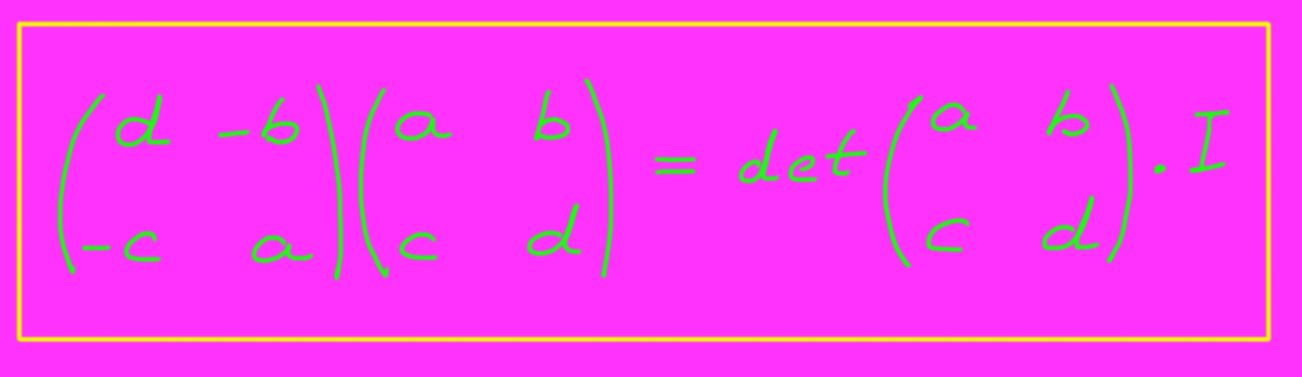
\includegraphics[scale=.2]{\propDetPath/adj2x2.jpg}
%\end{center}
%\end{figure}
Or in a more careful notation: if
\[M=\begin{pmatrix}
m^1_1 & m^1_2 \\[1mm]
m^2_1 & m^2_2 \\
\end{pmatrix}\, ,\] 
then \[M^{-1}=\frac{1}{m^1_1m^2_2-m^1_2m^2_1}\begin{pmatrix}
m^2_2 & -m^1_2 \\
-m^2_1 & m^1_1 \\
\end{pmatrix}\, ,\]
so long as $\det M=m^1_1m^2_2-m^1_2m^2_1\neq 0$.
  The  matrix $\begin{pmatrix}
m^2_2 & -m^1_2 \\
-m^2_1 & m^1_1 \\
\end{pmatrix}$ that appears above is a special matrix, called the \emph{adjoint} of $M$.  Let's define the adjoint for an $n \times n$ matrix.


The {\bfseries cofactor}\index{Cofactor} of $M$ corresponding to the entry $m^i_j$ of $M$ 
%and then deleting the $i$th row and $j$th column of $M$, taking the determinant of the 
is the product of the minor associated to $m^i_j$
%resulting matrix, and 
%multiplying by
and $(-1)^{i+j}$.  This is written $\cofactor(m^i_j)$.

\begin{definition}
For $M=(m^i_j)$ a square matrix, the {\bfseries adjoint matrix} $\adj M$ is given by
\[
\adj M = (\cofactor(m^i_j))^T.
\]
\end{definition}

\begin{example}
\[
\adj \begin{pmatrix}
3 & -1 & -1 \\
1 & 2 & 0 \\
0 & 1 & 1 \\
\end{pmatrix}
=
\begin{pmatrix}
\mc{\det \begin{pmatrix}
2 & 0 \\
1 & 1 
\end{pmatrix}}
& \mc{-\det \begin{pmatrix}
1 & 0 \\
0 & 1 
\end{pmatrix}}
&\mc{ \det \begin{pmatrix}
1 & 2 \\
0 & 1 
\end{pmatrix}}
\\[4mm]
-\det \begin{pmatrix}
-1 & -1 \\
1 & 1 
\end{pmatrix}
& \det \begin{pmatrix}
3 & -1 \\
0 & 1 
\end{pmatrix}
& -\det \begin{pmatrix}
3 & -1 \\
0 & 1 
\end{pmatrix}
\\[4mm]
\det \begin{pmatrix}
-1 & -1 \\
2 & 0 
\end{pmatrix}
& -\det \begin{pmatrix}
3 & -1 \\
1 & 0 
\end{pmatrix}
& \det \begin{pmatrix}
3 & -1 \\
1 & 2 
\end{pmatrix}
\\
\end{pmatrix}^T
\]
\end{example}

%\begin{center}\href{\webworkurl ReadingHomework14/2/}{Reading homework: problem 14.2}\end{center}
\Reading{Determinants}{6}

Let's compute the product $M\adj M$.  For any matrix $N$, the $i, j$ entry of $MN$ is given by taking the dot product of the $i$th row of $M$ and the $j$th column of $N$.  
Notice that the dot product of the $i$th row of $M$ and the $i$th column of $\adj M$ is just the expansion by minors of $\det M$ in the $i$th row.
Further, notice that the dot product of the $i$th row of $M$ and the $j$th column of $\adj M$ with $j\neq i$ is the same as expanding $M$ by minors, but with the $j$th row replaced by the $i$th row.  Since the determinant of any matrix with a row repeated is zero, then these dot products are zero as well.

We know that the $i,j$ entry of the product of two matrices is the dot product of the $i$th row of the first by the $j$th column of the second.  Then:
\[
M\adj M = (\det M) I
\]

Thus, when $\det M\neq 0$, the adjoint gives an explicit formula for $M^{-1}$.


\begin{theorem}
For $M$ a square matrix with $\det M\neq 0$ (equivalently, if $M$ is invertible), then
\[
M^{-1}=\frac{1}{\det M}\adj M
\]
\end{theorem}

\videoscriptlink{properties_of_determinant_adjoint.mp4}{The Adjoint Matrix}{video_properties_of_determinant_adjoint}


\begin{figure}
\begin{center}

\includegraphics[scale=.3]{\propDetPath/adjM.jpg}
\end{center}
\end{figure}

\begin{example}
Continuing with the previous example,
\[
\adj \begin{pmatrix}
3 & -1 & -1 \\
1 & 2 & 0 \\
0 & 1 & 1 \\
\end{pmatrix} = \begin{pmatrix}
2 & 0 & 2 \\
-1 & 3 & -1 \\
1 & -3 & 7 \\
\end{pmatrix}.
\]

Now, multiply:

\begin{eqnarray*}
\begin{pmatrix}
3 & -1 & -1 \\
1 & 2 & 0 \\
0 & 1 & 1 \\
\end{pmatrix}
\begin{pmatrix}
2 & 0 & 2 \\
-1 & 3 & -1 \\
1 & -3 & 7 \\
\end{pmatrix}
&=&
\begin{pmatrix}
6 & 0 & 0 \\
0 & 6 & 0 \\
0 & 0 & 6 \\
\end{pmatrix} \\[1mm]
\Rightarrow \begin{pmatrix}
3 & -1 & -1 \\
1 & 2 & 0 \\
0 & 1 & 1 \\
\end{pmatrix}^{-1} & = & \frac{1}{6}\begin{pmatrix}
2 & 0 & 2 \\
-1 & 3 & -1 \\
1 & -3 & 7 \\
\end{pmatrix}
\end{eqnarray*}

This process for finding the inverse matrix is sometimes called \emph{Cramer's~Rule}~\index{Cramer's rule}.
\end{example}

\subsection{Application: Volume of a Parallelepiped}

Given three vectors $u,v,w$ in $\Re^3$, the parallelepiped\index{Parallelepiped} determined by the three vectors is the ``squished'' box whose edges are parallel to $u, v$, and $w$ as depicted in Figure~\ref{parallelepiped}.

You probably learnt in a  calculus course  that the volume of this object is $|u\dotprod (v\times w)|$.  This is the same as expansion by minors of the matrix whose columns are $u,v,w$.  Then:
\[
\text{Volume}=\big|\det \begin{pmatrix}u & v & w \end{pmatrix} \big|
\] 



\begin{figure}
\begin{center}
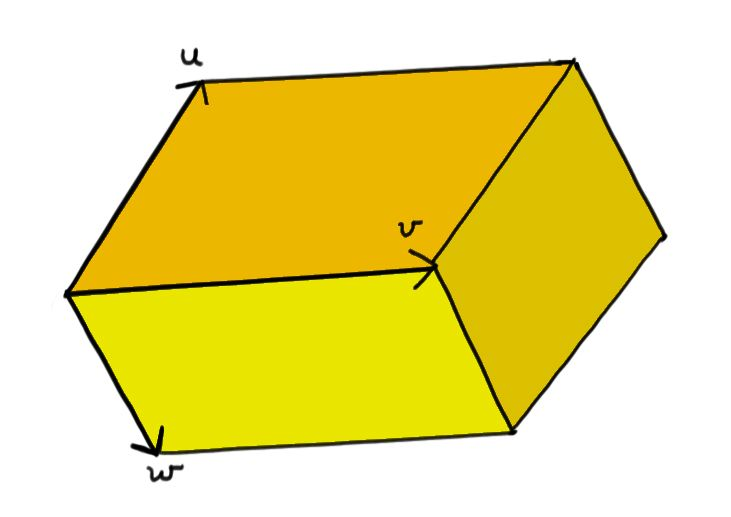
\includegraphics[scale=.4]{parallelepiped.jpg}
\caption{A parallelepiped.\label{parallelepiped}}
\end{center}
\end{figure}



%\section*{References}
%Hefferon, Chapter Four, Section I.1 and I.3
%\\
%Beezer, Chapter D, Section DM, Subsection DD
%\\
%Beezer, Chapter D, Section DM, Subsection CD
%\\
%Wikipedia:
%\begin{itemize}
%\item \href{http://en.wikipedia.org/wiki/Determinant}{Determinant}
%\item \href{http://en.wikipedia.org/wiki/Elementary_matrix}{Elementary Matrix}
%\item \href{http://en.wikipedia.org/wiki/Cramers_rule}{Cramer's Rule}
%\end{itemize}




\section{Review Problems}
{\bfseries Webwork:} 
\begin{tabular}{|c|c|}
\hline
Reading Problems & 
 \hwrref{Determinants}{5},\hwrref{Determinants}{6}\\
 Row of zeros & \hwref{Determinants}{12}\\
 $3\times 3$ determinant & \hwref{Determinants}{13}\\
 Triangular determinants & \hwref{Determinants}{14},\hwref{Determinants}{15},\hwref{Determinants}{16},\hwref{Determinants}{17}\\
Expanding in a column & \hwref{Determinants}{18}\\ 
 Minors and cofactors & \hwref{Determinants}{19}\\
 \hline
\end{tabular}






\begin{enumerate}
\item \label{det33} Let $M=\begin{pmatrix}
m^1_1 & m^1_2 & m^1_3\\
m^2_1 & m^2_2 & m^2_3\\
m^3_1 & m^3_2 & m^3_3\\
\end{pmatrix}$.  Use row operations to put $M$ into \emph{row echelon form}.  For simplicity, assume that $m_1^1\neq 0 \neq m^1_1m^2_2-m^2_1m^1_2$.

Prove that $M$ is non-singular if and only if:
\[
m^1_1m^2_2m^3_3 
- m^1_1m^2_3m^3_2 
+ m^1_2m^2_3m^3_1 
- m^1_2m^2_1m^3_3 
+ m^1_3m^2_1m^3_2
- m^1_3m^2_2m^3_1
\neq 0
\]

\phantomnewpage

\item 
\begin{enumerate}
\item What does the matrix $E^1_2=\begin{pmatrix}
0 & 1 \\
1 & 0
\end{pmatrix}$ do to $M=\begin{pmatrix}
a & b \\
d & c
\end{pmatrix}$ under left multiplication?  What about right multiplication?
\item Find elementary matrices $R^1(\lambda)$ and $R^2(\lambda)$ that respectively multiply rows $1$ and $2$ of $M$ by $\lambda$ but otherwise leave $M$ the same under left multiplication.
\item Find a matrix $S^1_2(\lambda)$ that adds a multiple $\lambda$ of row $2$ to row $1$ under left multiplication.
\end{enumerate}

\phantomnewpage

\item Let $M$ be a matrix and $S^i_jM$ the same matrix with rows \(i\) and \(j\) switched.  Explain every line of the 
\hyperlink{rowswap}{series of equations} proving that $\det M = -\det (S^i_jM)$.

\phantomnewpage

%\item \label{prob_inversion_number} This problem is a ``hands-on'' look at why \hyperlink{permutation_parity}{the property} describing the parity of permutations is true.
%
%\hypertarget{inversion_number}{The \emph{inversion number}}\index{Permutation!Inversion number} of a permutation $\sigma$ is the number of pairs $i<j$ such that $\sigma(i)>\sigma(j)$; it's the number of ``numbers that appear left of smaller numbers'' in the permutation.  For example, for the permutation $\rho = [4,2,3,1]$, the inversion number is $5$. The number $4$ comes before $2,3,$ and $1$, and $2$ and $3$ both come before $1$.
%
%Given a permutation $\sigma$, we can make a new permutation $\tau_{i,j} \sigma$ by exchanging the $i$th and $j$th entries of $\sigma$.
%
%\begin{enumerate}
%\item What is the inversion number of the permutation \(\mu=[1,2,4,3]\) that exchanges 4 and 3 and leaves everything else alone? Is it an even or an odd permutation?
%
%\item What is the inversion number of the permutation \(\rho=[4,2,3,1]\) that exchanges 1 and 4 and leaves everything else alone? Is it an even or an odd permutation?
%
%\item What is the inversion number of the permutation \(\tau_{1,3} \mu\)? Compare the parity\footnote{The \emph{parity} of an integer refers to whether the integer is even or odd. Here the parity of a permutation $\mu$ refers to the parity of its inversion number.} of \(\mu\) to the parity of \(\tau_{1,3} \mu.\)
%
%\item What is the inversion number of the permutation \(\tau_{2,4} \rho\)? Compare the parity of \(\rho\) to the parity of \(\tau_{2,4} \rho.\)
%
%\item What is the inversion number of the permutation \(\tau_{3,4} \rho\)? Compare the parity of \(\rho\) to the parity of \(\tau_{3,4} \rho.\)
%\end{enumerate}
%
%\videoscriptlink{elementary_matrices_determinant_hint.mp4}{Problem~\ref{prob_inversion_number} hints}{scripts_elementary_matrices_determinants_hint}

\phantomnewpage

%\item \label{problem_permutation} (Extra credit) Here we will examine a (very) small set of the general properties about permutations and their applications. In particular, we will show that one way to compute the sign of a permutation is by finding the \hyperlink{inversion_number}{inversion number} $N$ of $\sigma$ and we have
%\[
%\sgn(\sigma) = (-1)^N.
%\]
%
%For this problem, let $\mu = [1,2,4,3]$.
%
%\begin{enumerate}
%\item Show that every permutation $\sigma$ can be sorted by only taking simple (adjacent) transpositions\index{Permutation!Simple transposition} $s_i$ where $s_i$ interchanges the numbers in position $i$ and $i+1$ of a permutation $\sigma$ (in our other notation $s_i = \tau_{i,i+1}$). For example $s_2 \mu = [1, 4, 2, 3]$, and to sort $\mu$ we have $s_3 \mu = [1, 2, 3, 4]$.
%
%\item \label{prob_part_relations} We can compose simple transpositions together to represent a permutation (note that the sequence of compositions is not unique), and these are associative, we have an identity (the trivial permutation where the list is in order or we do nothing on our list), and we have an inverse since it is clear that $s_i s_i \sigma = \sigma$. Thus permutations of $[n]$ under composition are an example of a \hyperref[groups]{group}. However note that not all simple transpositions commute with each other since
%\begin{align*}
%s_1 s_2 [1, 2, 3] & = s_1 [1, 3, 2] = [3, 1, 2]
%\\ s_2 s_1 [1, 2, 3] & = s_2 [2, 1, 3] = [2, 3, 1]
%\end{align*}
%(you will prove here when simple transpositions commute). When we consider our initial permutation to be the trivial permutation $e = [1, 2, \dotsc, n]$, we do not write it; for example $s_i \equiv s_i e$ and $\mu = s_3 \equiv s_3 e$. This is analogous to not writing 1 when multiplying. Show that $s_i s_i = e$ (in shorthand $s_i^2 = e$), $s_{i+1} s_i s_{i+1} = s_i s_{i+1} s_i$ for all $i$, and $s_i$ and $s_j$ commute for all $|i - j| \geq 2$.
%
%\item Show that every way of expressing $\sigma$ can be obtained from using the relations proved in part~\ref{prob_part_relations}. In other words, show that for any expression $w$ of simple transpositions representing the trivial permutation $e$, using the proved relations.
%
%\emph{Hint: Use induction on $n$. For the induction step, follow the path of the $(n+1)$-th strand by looking at $s_n s_{n-1} \cdots s_k s_{k\pm1} \cdots s_n$ and argue why you can write this as a subexpression for any expression of $e$. Consider using diagrams of these paths to help.}
%
%\item The simple transpositions \hyperlink{action}{acts on} an $n$-dimensional vector space $V$ by $s_i v = E^i_{i+1} v$ (where $E^i_j$ is \hyperlink{elem_matrix_row_swap}{an elementary matrix}) for all vectors $v \in V$. Therefore we can just represent a permutation $\sigma$ as the matrix $M_{\sigma}$\footnote{Often people will just use $\sigma$ for the matrix when the context is clear.}, and we have $\det(M_{s_i}) = \det(E^i_{i+1}) = -1$. Thus prove that $\det(M_{\sigma}) = (-1)^N$ where $N$ is a number of simple transpositions needed to represent $\sigma$ as a permutation. You can assume that $M_{s_i s_j} = M_{s_i} M_{s_j}$ (it is not hard to prove) and that $\det(A B) = \det(A) \det(B)$ \hyperref[detmultiplicative]{from Chapter~\ref*{elementarydeterminantsII}}.
%
%\emph{Hint: You to make sure $\det(M_{\sigma})$ is well-defined since there are infinite ways to represent $\sigma$ as simple transpositions.}
%
%\item Show that $s_{i+1} s_i s_{i+1} = \tau_{i, i+2}$, and so give one way of writing $\tau_{i, j}$ in terms of simple transpositions? Is $\tau_{i,j}$ an even or an odd permutation? What is $\det(M_{\tau_{i,j}})$? What is the inversion number of $\tau_{i,j}$?
%
%\item The minimal number of simple transpositions needed to express $\sigma$ is called the \emph{length}\index{Permutation!Length} of $\sigma$; for example the length of $\mu$ is 1 since $\mu = s_3$. Show that the length of $\sigma$ is equal to the inversion number of $\sigma$.
%
%\emph{Hint: Find an procedure which gives you a new permutation $\sigma^{\prime}$ where $\sigma = s_i \sigma^{\prime}$ for some $i$ and the inversion number for $\sigma^{\prime}$ is 1 less than the inversion number for $\sigma$.}
%
%\item Show that $(-1)^N = \sgn(\sigma) = \det(M_{\sigma})$, where $\sigma$ is a permutation with $N$ inversions. Note that this immediately implies that $\sgn(\sigma \rho) = \sgn(\sigma) \sgn(\rho)$ for any permutations $\sigma$ and $\rho$.
%\end{enumerate}

\item Let $M'$ be the matrix obtained from $M$ by swapping two columns $i$ and $j$. Show that $\det M'=-\det M $.

\item The scalar triple product of three vectors $u,v,w$ from $\Re^3$ is $u\cdot(v\times w)$. Show that this product is the same as the determinant of the matrix whose columns are $u,v,w$ (in that order). What happens to the scalar triple product when the factors are permuted? 

\item Show that if $M$ is a $3\times 3$ matrix whose third row is a sum of multiples of the other rows ($R_3=aR_2+bR_1$) then $\det M=0$. Show that the same is true if one of the columns is a sum of multiples of the others. 

\end{enumerate}

\phantomnewpage

\newpage














